% comando para correção ortográfica
%$ aspell -t -c introducao.tex --encoding=utf-8 --lang=pt_BR

\chapter{Introdução}

\section{Problemática}
O consumo de jogos é crescente nos últimos 5 anos, como podemos ver na figura
\ref{fig:esa_graph_2017} das pesquisas da ESA,
segundo os mesmos, em 2016 o consumidor norte americano gastou em torno de $30.4$
bilhões de dólares na industria dos jogos. No mesmo ano, as companhias de jogos
norte americanas adicionaram mais de 11.7 bilhões de dólares na \textit{GDP}
do país \cite{entertainment2017essential}.
\begin{figure}[H]
    \centering
    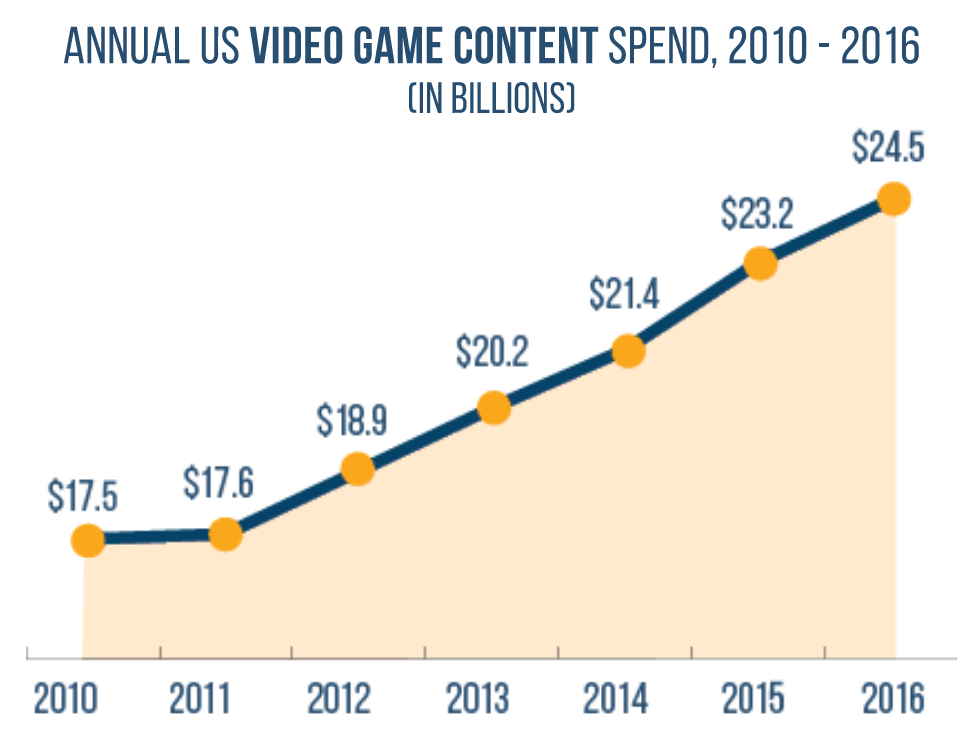
\includegraphics[width=0.5\textwidth]{figuras/ESAGraph2017.png}
    \caption{Consumo com conteúdo de jogos\cite{entertainment2017essential}}
    \label{fig:esa_graph_2017}
\end{figure}

Em contrapartida, os investimentos nos jogos também são crescentes neste
período \cite{entertainment2017essential}, um dos jogos com mais investimentos é
o \textit{GTAV} que em desenvolvimento e marketing gastou cerca de $265$
milhões de dólares \cite{villapaz2013gta}. Os jogos tendem a ser cada vez mais,
detalhados e complexos, desta maneira o custo de desenvolvimento também aumenta.
No desenvolvimento de jogos temos vários profissionais envolvidos para criar
o conteúdo dos jogos, com equipes de programadores, designers,  roteiristas,
entre outros. A força de trabalho dos mesmos costuma ser a parte mais cara da
criação do jogo.

\section{Apresentação}
O trabalho em questão tem a finalidade de avaliar algumas características
de relevo, como planícies e cordilheiras, implementar um algoritmo sem 
interferência do usuário, que forme proceduralmente o relevo destas características.
O relevo precisa ser contínuo quando houver fronteira ou transição de uma para 
a outra. O tamanho do mapa deve ser pseudo-infinito e carregar apenas regiões
próximas da câmera.

Uma maneira de conseguir diminuir os gastos no desenvolvimento de conteúdo, é 
gerando os mesmos proceduralmente, as chamadas técnicas de \textit{PCG}. 
\textit{PCG} é usar algoritmos para gerar o conteúdo \cite{shaker2016procedural}.
Uma aplicação bem comum do \textit{PCG} é a criação de relevos e mapas de altura,
desta maneira não é necessário uma pessoa modelar manualmente a altura do
terreno do cenário.

Com o \textit{PCG} para criar o terreno, é possível criar eles com tamanhos
pseudo-infinitos, hoje temos diversos exemplos de jogos que fazem uso dessa técnica
para criar um cenário pseudo-infinitos, entre eles, \textit{Limit Theory}, nele
são criados pseudo-infinitos sistemas planetários, de forma procedural, e em cada
sistema planetário os planetas e seus relevos também são gerados proceduralmente
\cite{abreu1990toward}.

O algoritmo para criar o terreno deve ser implementado conforme as
características do bioma alvo, como exemplo, a implementação de 
\cite{gabrielle2016canion} e \cite{carli2012canion}, ambos geram relevos de
cânions, como podemos visualizar na figura \ref{fig:carli2012result}.
\begin{figure}[H]
    \centering
    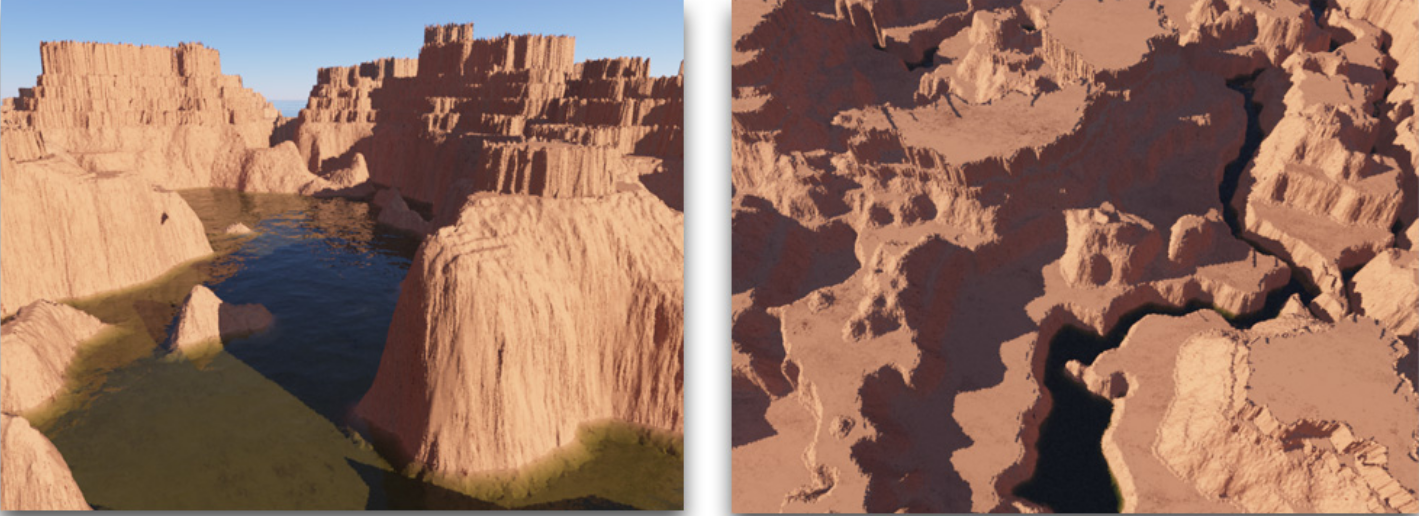
\includegraphics[width=0.9\textwidth]{figuras/carli2012result.png}
    \caption{Resultado do trabalho de \cite{carli2012canion}}
    \label{fig:carli2012result}
\end{figure}

Na técnica de \cite{patel2010polygonal}, que gera ilha proceduralmente, cada uma podendo ter
múltiplos biomas. Para começar é criado um diagrama de Voronoi, onde cada \textit{site}
vai representar uma região do mapa, os \textit{sites} são gerados em posições
aleatórias, seguido por Lloyd's algorithm no diagrama para
deixar as regiões mais relaxadas.
Então é usados uma sequencia de ruídos bidimensionais sobre o mapa para decidir
áreas de oceano ou ilha, altura da região e bioma da região, seguido por funções
de ruídos unidimensionais para as bordas da ilha e fronteiras das regiões ter
uma aparência mais natural, por fim tendo como resultado final ilustrado na
figura \ref{fig:voronoi-map-goal-distorted}.
\begin{figure}[H]
    \centering
    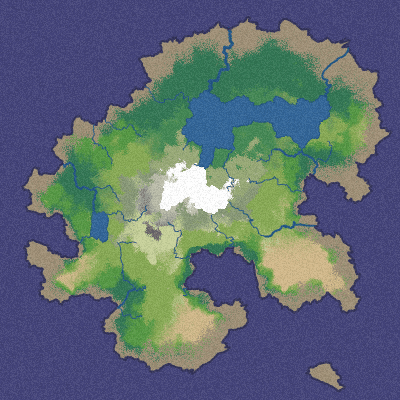
\includegraphics[width=0.4\textwidth]{figuras/voronoi-map-goal-distorted.png}
    \caption{Resultado final de \cite{patel2010polygonal}}
    \label{fig:voronoi-map-goal-distorted}
\end{figure}

O jogo \textit{minecraft} tem uma implementação de geração procedural,
seus mundos são de tamanho pseudo-infinito, 
o algoritmo é não assistido, ou seja, sem a intervenção
do usuário na criação do mundo, nele
são gerados múltiplos biomas, em cada um deles existe uma manipulação diferente
do ruído para recriar as características do bioma. Mesmo em seu mundo
minimalista, o jogador consegue reconhecer o bioma \cite{short2012teaching},
como na figura \ref{fig:biomesminecraftgameplay}.
Foi usado o sistema online \textit{Chunck Base} para 
ilustrar fronteiras entre biomas, cada cor no mapa é um bioma \ref{fig:chunkbasebiomes}.


\begin{figure}[H]
    \centering
    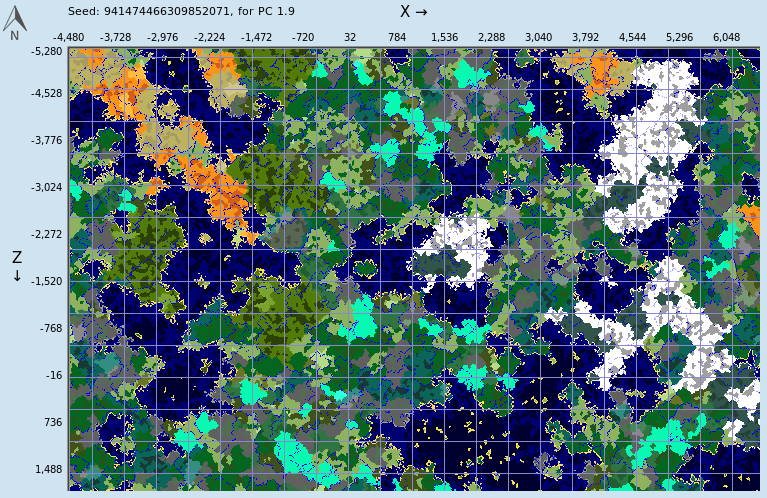
\includegraphics[width=0.7\textwidth]{figuras/chunkbasebiomes.png}
    \caption{Mapa de biomas para mundo virtual do \textit{minecraft}}
    \label{fig:chunkbasebiomes}
\end{figure}

\begin{figure}[H]
    \centering
    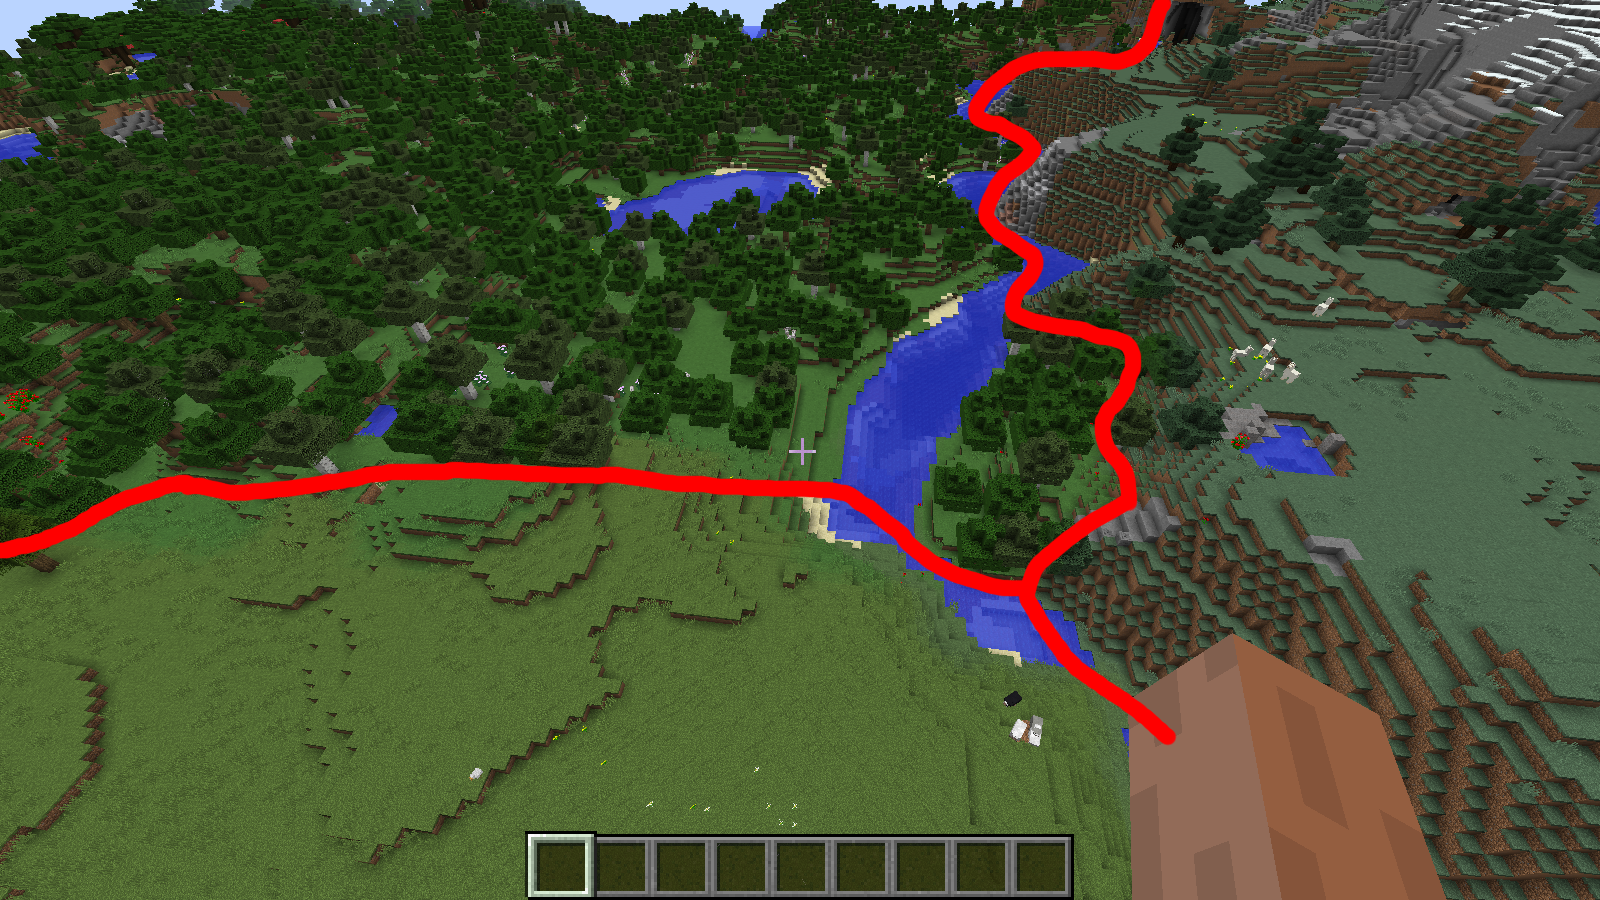
\includegraphics[width=0.7\textwidth]{figuras/biomesminecraftgameplay.png}
    \caption{Perspectiva de um jogador no \textit{minecraft}, com visão para fronteira entre três biomas}
    \label{fig:biomesminecraftgameplay}
\end{figure}

\section{Objetivo Geral}
Este projeto tem como objetivo gerar mapas de tamanho pseudo-infinitos, com 
relevo gerado proceduralmente usando ruído 
de Perlin, de maneira não assistida, os mapas de altura devem representar o 
relevo de pelo menos dois biomas arbitrários com fronteiras contínuas.

%Criar um método procedural para múltiplos biomas ter fronteiras contínuas

\section{Objetivo Específico}

\begin{itemize}
    \item Implementar malhas da superfície com tamanho pseudo-infinito;
    \item Selecionar biomas, e as características dos mesmos a ser representadas;
    \item Construir algoritmo para manipular ruído de Perlin e gerar características
        selecionadas do bioma;
    \item Gerar divisões entre biomas sobre a malha de regiões;
    \item Implementar fronteiras contínuas entre biomas;
    \item Comparar resultado com cenários de jogos;
\end{itemize}
%\subsubsection{Exemplo de ilustração}

%\begin{figure}[h]
%\captionsetup{justification=raggedright, singlelinecheck=false}
%\centering
%
\includegraphics[scale=0.4]{figuras/uffs.eps}
%\caption{Exemplo de ilustração.}
%\label{fig:uffs}
%\end{figure}



%Exemplo do Matheus
%\begin{figure}[H]
%  \centering
%  \includegraphics[width=0.9\textwidth]{figuras/tcc2/pts_sem_peso/evento_de_site_insercao_fronteiras.png}
%  \caption{ES para o \textit{site} $s$.}
%  \label{fig:cenario_insercao_de_fronteiras}
%\end{figure}
%
%  Levando em consideração o cenário da figura \ref{fig:cenario_insercao_de_fronteiras}, 
%$s$ está contido em $R^{*}_{q}$, portanto serão criadas as fronteiras $C^{-}_{qs}$ e $C^{+}_{qs}$,
